\documentclass[11pt,a4paper,notitlepage,onecolumn]{article}
\usepackage[german]{babel}
\usepackage[utf8]{inputenc}
\usepackage{graphicx}
\title{Aufgabe5\_3}
\author{Robin Nehls, Yves Müller\\
  Freie Universit\"at Berlin\\
  nehls@spline.de uves@spline.de }
\date{}
\begin{document}

\maketitle

\paragraph{Comparison to analyical solution}
Actually we were not able to put the analytical solution together, due to a
leck understanding in quantum physics. So we are not able to make an 
quntitative comaprison. But a qulatativ compersion to a paper 
(http://www.jkrieger.de/download/quantenmechanik.pdf/ p. 67) shows that our
results are pretty close to the analytic solution. We assume that a better 
result could be reach by choosing smaller $\Delta x$ for the discretisation.


\paragraph{}


\begin{figure}
\centering
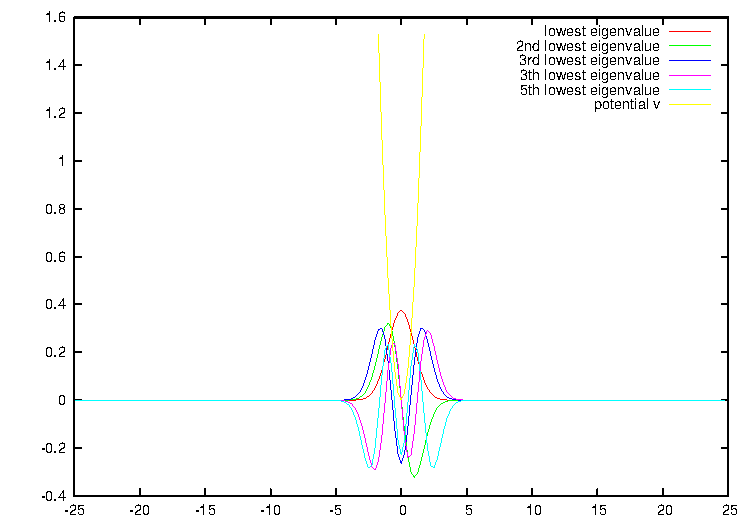
\includegraphics[width=\textwidth]{aufgabe3-normal.pdf}
\caption{\em \small plott of the lowest 5 eigenvalues}
\end{figure}

\paragraph{Choosing smaller harmonic potentials}
When computing the hamiltonien with smaller potentials, we meet several new 
problems. First of all our solutions have much smaller absolute values, but
our machine accuraccy keeps still the same, wich leavs might lead to bigger
relative Error. On the other hand we have to increase the our N or increase 
our $\Delta x$, in order to be able to plot all eigenfunctions completle,
wich results in more operations (where $O(n)=n^3$), or lesser accuracy. If 
the potential is choosen very low the longitude of the ozzilator is growing
fast.

\begin{figure}
\centering
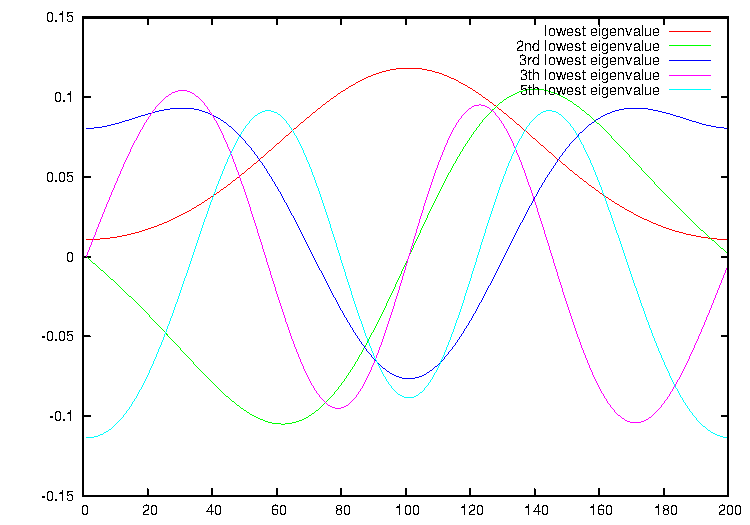
\includegraphics[width=\textwidth]{aufgabe3-lowpot.pdf}
\caption{\em \small plot with lower harmonic potential}
\end{figure}



\end{document}
